\documentclass[11pt,a4paper]{ctexart}
\usepackage{ipara}
\tcbuselibrary{breakable}
\usetikzlibrary{arrows.meta,positioning}

\pagestyle{fancy}
\fancyhf{}
\lhead{\small 高中数学专题研究}
\rhead{\small 复合方程根的个数问题讨论}
\cfoot{\small 第 \thepage\ 页\quad 共 \zpageref{LastPage} 页}
\renewcommand{\headrulewidth}{0.4pt}
\renewcommand{\footrulewidth}{0pt}

\begin{document}

\begin{center}
  {\zihao{2}\bfseries 复合方程实根个数问题的分类讨论}\\[3mm]
  {\large ——一类分段超越复合方程的经典解析}\\[2mm]
  \rule{0.85\linewidth}{0.5pt}
\end{center}

在高考及各类数学竞赛中，含有分段函数与超越函数的复合方程根的个数问题是一类极其重要的代数综合题。解决此类问题的核心思想在于\textbf{换元法与等价转化}，即通过引入中间变量将复合方程拆解为外层代数方程与内层对应方程，再结合函数图像进行分类讨论。

\begin{exbox}{【例题】}
已知函数
\[
f(x)=
\begin{cases}
x^2+2x+2,\quad x\le 0,\\
|\ln x-1|,\quad x>0,
\end{cases}
\]
若关于 \(x\) 的方程
\[
a[f(x)]^2-(3a+1)f(x)+5=0
\]
有 6 个不相等的实数根，求实数 \(a\) 的取值范围。
\end{exbox}

\section{解析与图像分析}

\subsection{第一步：内层自变量换元与根的映射分析}

令中间变量为 \(t = f(x)\)，则原复合方程可等价转化为关于 \(t\) 的外层方程：
\[
at^2-(3a+1)t+5=0. \tag{1}
\]
为了确定方程 (1) 的根对应的原方程 \(x\) 根的个数，我们必须系统分析内层方程 \(f(x) = t\) 在不同实数 \(t\) 下的实根个数。

对于分段函数 \(f(x)\)：
\begin{enumerate}
  \item 当 \(x \le 0\) 时，\(f(x) = x^2 + 2x + 2 = (x+1)^2 + 1\)。这是一段抛物线，其对称轴为 \(x = -1\)，顶点坐标为 \((-1, 1)\)。在此区间内，\(f(x)\) 的最小值为 1。
  \item 当 \(x > 0\) 时，\(f(x) = |\ln x - 1|\)。这是一段含有绝对值的对数曲线，其值域为 \([0, +\infty)\)。在 \(x = e\) 处取得最小值 0（为图像的折返尖点）。
\end{enumerate}

为便于直观观测，我们绘制函数 \(f(x)\) 的图像，并作水平参考线 \(y = t\) 如下：

\begin{center}
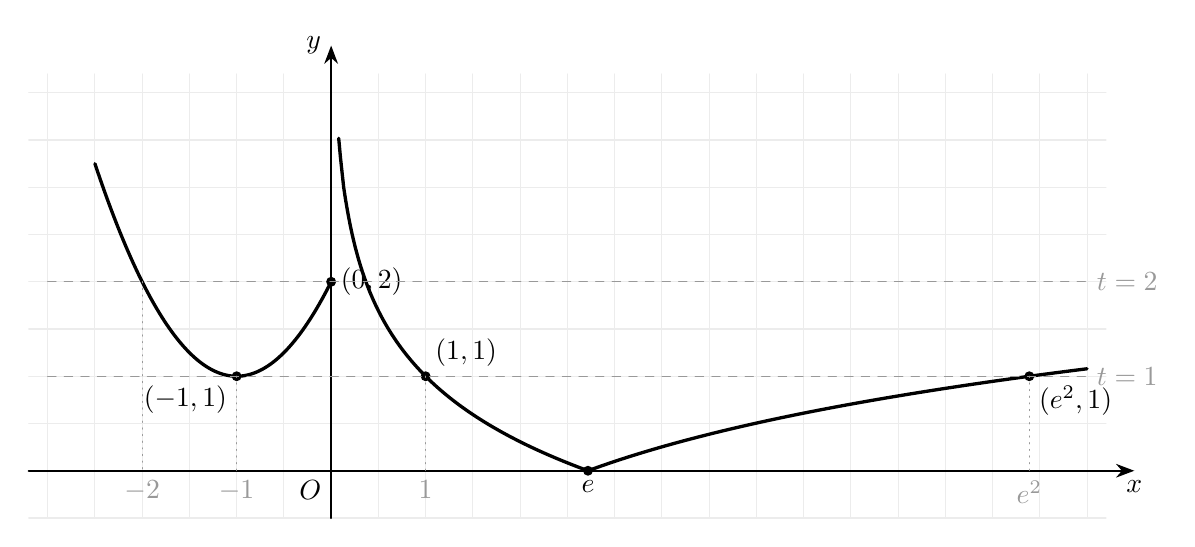
\begin{tikzpicture}[scale=1.2, >=Stealth, line join=round, line cap=round]
  % 网格辅助线
  \draw[color=gray!15, thin, step=0.5] (-3.2,-0.5) grid (8.2,4.2);
  
  % 坐标轴
  \draw[->, thick] (-3.2,0) -- (8.5,0) node[below] {\(x\)};
  \draw[->, thick] (0,-0.5) -- (0,4.5) node[left] {\(y\)};
  \node[below left] at (0,0) {\(O\)};
  
  % 绘制函数 f(x)
  \draw[domain=-2.5:0, samples=100, very thick, color=black] plot (\x, {\x*\x + 2*\x + 2});
  \draw[domain=0.08:2.718, samples=150, very thick, color=black] plot (\x, {1 - ln(\x)});
  \draw[domain=2.718:8.0, samples=150, very thick, color=black] plot (\x, {ln(\x) - 1});
  
  % 关键点标记与坐标
  \fill[black] (-1,1) circle (1.5pt) node[below left] {\((-1,1)\)};
  \fill[black] (0,2) circle (1.5pt) node[right] {\((0,2)\)};
  \fill[black] (1,1) circle (1.5pt) node[above right] {\((1,1)\)};
  \fill[black] (2.718,0) circle (1.5pt) node[below] {\(e\)};
  \fill[black] (7.389,1) circle (1.5pt) node[below right] {\((e^2,1)\)};
  
  % t = 1 和 t = 2 的水平参考线
  \draw[dashed, color=gray!80, thin] (-3.0,1) -- (8.0,1) node[right] {\(t=1\)};
  \draw[dashed, color=gray!80, thin] (-3.0,2) -- (8.0,2) node[right] {\(t=2\)};
  
  % 投影线到 x 轴
  \draw[dotted, color=gray!80] (-1,1) -- (-1,0) node[below] {\(-1\)};
  \draw[dotted, color=gray!80] (1,1) -- (1,0) node[below] {\(1\)};
  \draw[dotted, color=gray!80] (7.389,1) -- (7.389,0) node[below] {\(e^2\)};
  \draw[dotted, color=gray!80] (-2,2) -- (-2,0) node[below] {\(-2\)};
\end{tikzpicture}
\\
\textbf{图 1：函数 \(f(x)\) 图像与参数水平线 \(t\) 交点数分析示意图}
\end{center}

通过数形结合，考查水平直线 \(y=t\) 与函数 \(f(x)\) 图像的交点个数，可以得出自变量 \(t\) 与对应实根 \(x\) 个数的完整映射表：

\begin{center}
\renewcommand{\arraystretch}{1.4}
\begin{tabularx}{\textwidth}{c|c|X}
\hline
\(t\) 的取值范围 & \(f(x)=t\) 的实根个数 & 对应的实根具体分布 \\ \hline
\(t < 0\) & 0 & 无解 \\ 
\(t = 0\) & 1 & 唯一根为 \(x = e\) \\ 
\(0 < t < 1\) & 2 & 两根均分布在区间 \((0, +\infty)\) 内 \\ 
\(t = 1\) & 3 & 三根分别为 \(x = -1, x = 1, x = e^2\) \\ 
\(1 < t \le 2\) & 4 & 两根在区间 \((-\infty, 0]\) 内，另两根在区间 \((0, +\infty)\) 内 \\ 
\(t > 2\) & 3 & 一根在区间 \((-\infty, 0]\) 内，另两根在区间 \((0, +\infty)\) 内 \\ \hline
\end{tabularx}
\end{center}

因此，原方程有 6 个不相等的实数根，等价于关于 \(t\) 的方程 (1) 在非负半轴 \(t \ge 0\) 上的实根所对应的 \(x\) 根数总和恰好为 6。

\subsection{第二步：外层方程根的初步讨论}

设二次函数 \(Q(t) = at^2 - (3a+1)t + 5\)。我们首先对外层二次方程的系数 \(a\) 进行初步的讨论：
\begin{enumerate}[label=(\arabic*)]
  \item \textbf{若 } \(a = 0\)：
    方程 (1) 退化为一次方程 \(-t + 5 = 0\)，解得唯一的实根 \(t = 5\)。
    由上表可知，当 \(t = 5 > 2\) 时，方程 \(f(x) = 5\) 仅有 3 个不相等的实数根，与题设不符。
  \item \textbf{若 } \(a < 0\)：
    由于二次方程 \(Q(t) = 0\) 的常数项为 5，其两根之积为 \(\frac{5}{a} < 0\)，故方程必有一正根与一负根。
    其中，负根 \(t < 0\) 对应的内层方程 \(f(x) = t\) 无实数解；
    正根 \(t > 0\) 对应的内层方程 \(f(x) = t\) 最多产生 4 个实数解。
    因此，当 \(a < 0\) 时，原方程的实数根总个数最多为 4，与题设不符。
  \item \textbf{若 } \(a > 0\)：
    方程 (1) 为开口向上的二次方程，两根之积 \(\frac{5}{a} > 0\)，两根之和 \(\frac{3a+1}{a} > 0\)，若方程有实根，则必为两正根。
    为使方程有实根，其判别式必须满足：
    \[
    \Delta = (3a+1)^2 - 20a = 9a^2 - 14a + 1 > 0.
    \]
    解得实数 \(a\) 的范围为：
    \[
    a < \frac{7-2\sqrt{10}}{9} \quad \text{或} \quad a > \frac{7+2\sqrt{10}}{9}.
    \]
    结合 \(a > 0\) 的前提条件，初步确定 \(a\) 的允许区间为：
    \[
    a \in \left( 0, \frac{7-2\sqrt{10}}{9} \right) \cup \left( \frac{7+2\sqrt{10}}{9}, +\infty \right).
    \]
\end{enumerate}

\subsection{第三步：系数 \(a\) 范围的分类细化与精确配图讨论}

在此允许区间内，方程 (1) 必有两个不同的正实数根 \(t_1, t_2\)（因两根之积 \(\frac{5}{a} > 0\)，两根之和 \(\frac{3a+1}{a} > 0\)）。我们针对 \(a\) 所在的两个区间分别进行讨论。

\subsubsection{第一类情况：\(0 < a < \frac{7-2\sqrt{10}}{9}\)}

在此范围内，我们考查两根与边界值 2 的大小关系。令 \(t = u + 2\)，则方程 \(Q(t) = 0\) 转化为关于 \(u\) 的新方程：
\[
Q(u+2) = a(u+2)^2 - (3a+1)(u+2) + 5 = au^2 + (a-1)u + 3-2a = 0.
\]
其两个实根 \(u_1, u_2\) 满足根与系数的关系：
\[
u_1 + u_2 = \frac{1-a}{a} > 0, \quad \left( \text{因 } a < \frac{7-2\sqrt{10}}{9} \approx 0.075 < 1 \right)
\]
\[
u_1 u_2 = \frac{3-2a}{a} > 0. \quad \left( \text{因 } 2a < 1 < 3 \right)
\]
由此可知，方程的两个根 \(u_1, u_2\) 均为正数，从而方程 (1) 的两个正根 \(t_1, t_2\) 均满足：
\[
t_1 > 2, \quad t_2 > 2.
\]
由映射关系可知，每个大于 2 的 \(t\) 均对应 3 个不相等的 \(x\) 根。此时，原方程的实数根总个数为：
\[
3 + 3 = 6.
\]
此情况完全符合题意。对应的几何图像分析如图 2 所示。

\begin{center}
\begin{tikzpicture}[scale=1.2, >=Stealth, line join=round, line cap=round]
  % 网格辅助线
  \draw[color=gray!15, thin, step=0.5] (-3.2,-0.5) grid (8.2,4.2);
  
  % 坐标轴
  \draw[->, thick] (-3.2,0) -- (8.5,0) node[below] {\(x\)};
  \draw[->, thick] (0,-0.5) -- (0,4.5) node[left] {\(y\)};
  \node[below left] at (0,0) {\(O\)};
  
  % 绘制函数 f(x)
  \draw[domain=-2.5:0, samples=100, very thick, color=black] plot (\x, {\x*\x + 2*\x + 2});
  \draw[domain=0.08:2.718, samples=150, very thick, color=black] plot (\x, {1 - ln(\x)});
  \draw[domain=2.718:8.0, samples=150, very thick, color=black] plot (\x, {ln(\x) - 1});
  
  % 关键点
  \fill[black] (2.718,0) circle (1.2pt) node[below] {\(e\)};
  
  % t1 = 2.5
  \draw[dashed, color=red!80!black, thick] (-3.0,2.5) -- (8.0,2.5) node[right] {\(t_1\)};
  \fill[red!80!black] (-2.225,2.5) circle (1.8pt) node[above left] {\(x_1\)};
  \fill[red!80!black] (0.223,2.5) circle (1.8pt) node[above right] {\(x_2\)};
  \draw[->, color=red!80!black, >=Stealth] (7.5,2.5) -- (8.0,2.5); % 箭头指示右侧第3个根 (x3 = e^{3.5} 落在区域外)
  
  % t2 = 3.2
  \draw[dashed, color=blue!80!black, thick] (-3.0,3.2) -- (8.0,3.2) node[right] {\(t_2\)};
  \fill[blue!80!black] (-2.483,3.2) circle (1.8pt) node[above left] {\(x_4\)};
  \fill[blue!80!black] (0.111,3.2) circle (1.8pt) node[above right] {\(x_5\)};
  \draw[->, color=blue!80!black, >=Stealth] (7.5,3.2) -- (8.0,3.2); % 箭头指示右侧第6个根 (x6 = e^{4.2} 落在区域外)

  \node[draw, fill=white, font=\small] at (4,1.8) {\(t_1, t_2 > 2 \implies 3+3=6\) 个根};
\end{tikzpicture}
\\
\textbf{图 2：\(0 < a < \frac{7-2\sqrt{10}}{9}\) 时，两个 \(t\) 根均大于 2 对应 6 个实数根示意图}
\end{center}

\subsubsection{第二类情况：\(a > \frac{7+2\sqrt{10}}{9}\)}

在此范围内，两根的绝对分布区间被边界点所分割。我们通过计算关键边界处的函数值来锁定两根的分布区域：
\[
Q(1) = a - (3a+1) + 5 = 4 - 2a
\]
\[
Q(2) = 4a - 2(3a+1) + 5 = 3 - 2a
\]
\[
Q(3) = 9a - 3(3a+1) + 5 = 2 > 0.
\]
此外，二次函数 \(Q(t)\) 的对称轴为：
\[
t_{\text{轴}} = \frac{3a+1}{2a} = 1.5 + \frac{1}{2a} > 1.5.
\]
由此，我们对 \(a \in \left( \frac{7+2\sqrt{10}}{9}, +\infty \right)\) 细分以下情况进行讨论：

\begin{enumerate}[label=(\roman*)]
  \item \textbf{若 } \(\frac{7+2\sqrt{10}}{9} < a < \frac{3}{2}\)：\\
    此时 \(Q(1) > 0\)，\(Q(2) > 0\)，且对称轴位于区间 \((1.5, 2)\) 内。根据二次函数根的分布性质，两个不同的实根 \(t_1, t_2\) 均落在开区间 \((1, 2)\) 内。
    由映射表可知，每个在该区间内的 \(t\) 对应 4 个 \(x\) 的实数根。此时，原方程的实数根总个数为：
    \[
    4 + 4 = 8 \neq 6.
    \]
    此情况不符合题意。

  \item \textbf{若 } \(a = \frac{3}{2}\)：\\
    此时 \(Q(2) = 0\)，说明方程有一根为 \(t_2 = 2\)。代入方程求得另一根为 \(t_1 = \frac{4}{3} \in (1, 2)\)。
    根据映射表，\(t_2 = 2\) 对应 4 个实数根，\(t_1 = \frac{4}{3}\) 对应 4 个实数根。此时，原方程的实数根总个数为：
    \[
    4 + 4 = 8 \neq 6.
    \]
    此情况不符合题意。

  \item \textbf{若 } \(\frac{3}{2} < a < 2\)：\\
    此时 \(Q(1) > 0\)，\(Q(2) < 0\)，\(Q(3) > 0\)。说明方程的两个根分别落在区间：
    \[
    t_1 \in (1, 2), \quad t_2 \in (2, 3).
    \]
    根据映射表，\(t_1\) 对应 4 个实数根，\(t_2\) 对应 3 个实数根。此时，原方程的实数根总个数为：
    \[
    4 + 3 = 7 \neq 6.
    \]
    此情况不符合题意。

  \item \textbf{若 } \(a = 2\)：\\
    此时方程 (1) 转化为：
    \[
    2t^2 - 7t + 5 = (2t-5)(t-1) = 0.
    \]
    解得两个根分别为：
    \[
    t_1 = 1, \quad t_2 = 2.5.
    \]
    根据映射表，当 \(t_1 = 1\) 时，对应 3 个 \(x\) 的实数根（分别为 \(x = -1, 1, e^2\)）；当 \(t_2 = 2.5 > 2\) 时，对应 3 个 \(x\) 的实数根。
    此时，原方程的实数根总个数为：
    \[
    3 + 3 = 6.
    \]
    此情况完全符合题意。对应的几何图像分析如图 3 所示。

    \begin{center}
    \begin{tikzpicture}[scale=1.2, >=Stealth, line join=round, line cap=round]
      % 网格辅助线
      \draw[color=gray!15, thin, step=0.5] (-3.2,-0.5) grid (8.2,4.2);
      
      % 坐标轴
      \draw[->, thick] (-3.2,0) -- (8.5,0) node[below] {\(x\)};
      \draw[->, thick] (0,-0.5) -- (0,4.5) node[left] {\(y\)};
      \node[below left] at (0,0) {\(O\)};
      
      % 绘制函数 f(x)
      \draw[domain=-2.5:0, samples=100, very thick, color=black] plot (\x, {\x*\x + 2*\x + 2});
      \draw[domain=0.08:2.718, samples=150, very thick, color=black] plot (\x, {1 - ln(\x)});
      \draw[domain=2.718:8.0, samples=150, very thick, color=black] plot (\x, {ln(\x) - 1});
      
      % 关键点标记
      \fill[black] (2.718,0) circle (1.2pt) node[below] {\(e\)};
      
      % t1 = 1 (对应的3个交点)
      \draw[dashed, color=red!80!black, thick] (-3.0,1) -- (8.0,1) node[right] {\(t_1=1\)};
      \fill[red!80!black] (-1,1) circle (1.8pt) node[below left] {\(-1\)};
      \fill[red!80!black] (1,1) circle (1.8pt) node[above right] {\(1\)};
      \fill[red!80!black] (7.389,1) circle (1.8pt) node[below right] {\(e^2\)};
      
      % t2 = 2.5 (对应的3个交点)
      \draw[dashed, color=blue!80!black, thick] (-3.0,2.5) -- (8.0,2.5) node[right] {\(t_2=2.5\)};
      \fill[blue!80!black] (-2.225,2.5) circle (1.8pt) node[above left] {\(x'\)};
      \fill[blue!80!black] (0.223,2.5) circle (1.8pt) node[above right] {\(x''\)};
      \draw[->, color=blue!80!black, >=Stealth] (7.5,2.5) -- (8.0,2.5); % 箭头指向右侧第3个交点

      \node[draw, fill=white, font=\small] at (4,3.2) {\(t_1=1, t_2=2.5 \implies 3+3=6\) 个根};
    \end{tikzpicture}
    \\
    \textbf{图 3：\(a = 2\) 时，两正根分别为 \(1\) 和 \(2.5\) 对应 6 个实数根示意图}
    \end{center}

  \item \textbf{若 } \(a > 2\)：\\
    此时 \(Q(0) = 5 > 0\)，\(Q(1) < 0\)，\(Q(2) < 0\)，且 \(Q(3) > 0\)。由于对称轴介于 1 和 2 之间，方程的两个实根分布在区间：
    \[
    t_1 \in (0, 1), \quad t_2 \in (2, 3).
    \]
    根据映射表，\(t_1\) 对应 2 个实数根，\(t_2\) 对应 3 个实数根。此时，原方程的实数根总个数为：
    \[
    2 + 3 = 5 \neq 6.
    \]
    此情况不符合题意。
\end{enumerate}

\section{总结与结论}

\begin{theorembox}{本题结论}
综上所述，将所有符合题意的分类情况汇总，可得实数 \(a\) 的取值范围为：
\[
0 < a < \frac{7-2\sqrt{10}}{9} \quad \text{或} \quad a = 2.
\]
\end{theorembox}

\end{document}
